% +------------------------------------------------------------------------------------------------------------------+
%  Динамическое программирование: неэффективность ветвящейся рекурсии, оптимальная 
%  подструктура и пример её отсутствия, прямой и обратный ход метода динамического 
%  программирования, пример с числами Фибоначчи, пример с разложением в сумму квадратов                  
% +------------------------------------------------------------------------------------------------------------------+

\documentclass[a4paper,12pt] {report} 			% размер бумаги устанавливаем А4, шрифт 12пунктов
\usepackage{graphicx}						% подключаем графический модуль
\graphicspath{{pictures/}}						% путь к картинкам
\usepackage[utf8] {inputenc} 					% включаем свою кодировку: utf8 
\usepackage[english,russian] {babel} 			% используем русский и английский языки с переносами
\usepackage{misccorr}						% соответствие стандарту
\usepackage{tikz}								% подключаем модуль диаграмм
\usepackage{listingsutf8}						

\begin{document}

\begin{center}
	{\LARGE \bfseries \slshape Динамическое программирование}
\end{center}

{\bfseries Динамическое программирование}~--~способ решения сложных задач путём разбиения их на более простые подзадачи.

Часто многие из этих подзадач одинаковы. Подход динамического программирования состоит в том, чтобы 
решить каждую подзадачу только один раз, сократив тем самым количество вычислений.

\section{Рекурсивное решение}

Рассмотрим числа Фибоначчи. Они образуют последовательность $\{ F_{n}\}$, которая 
задается следующим рекурентным соотношением: $$F_{0} = 0, F_{1} = 1, F_{n} = F_{n-1} + F_{n-2}, n \ge 2, n \in Z$$

Проанализируем рекурсивный способ получения последовательности. Видно, что данный подход 
избыточен, так как значения $F_{i}$ высчитываются по несколько раз.

% <<<<реккурсивное дерево>>>>
\begin{center}
	\begin{tikzpicture}[level/.style={sibling distance=60mm/#1}]
	\node [circle,draw] {$F_{5}$}
		child{node [circle,draw] {$F_{4}$}
			child{node [circle,draw] {$F_{3}$}
				child{node {$\vdots$}}
				child{node {$\vdots$}}
			}
			child{node [circle,draw] {$F_{2}$}
				child{node {$\vdots$}}
				child{node {$\vdots$}}
			}
		}
		child{node [circle,draw] {$F_{3}$}
			child{node [circle,draw] {$F_{2}$}
				child{node {$\vdots$}}
				child{node {$\vdots$}}
			}
			child{node [circle,draw] {$F_{1}$}
				child{node {$\vdots$}}
				child{node {$\vdots$}}
			}
		};
	\end{tikzpicture}
\end{center}
% <<<<реккурсивное дерево>>>>

Приходим к тому, что количество действий в таком алгоритме тоже равно числу Фибоначчи. Воспользуемся 
формулой Бине, чтобы оценить скорость роста последовательности.

% <<<<формула Бине>>>>
$$F_{n} = \left(\frac{\left(\frac{1 + \sqrt{5}}{2}\right)^{n} - \left(\frac{1 - \sqrt{5}}{2}\right)^{n}}{\sqrt{5}}\right) $$
% <<<<формула Бине>>>>

Получаем, что скорость роста последовательности чисел фибоначчи: $O(\varphi^{n})$, где $\varphi = \frac{1 + \sqrt{5}}{2}$. 
Рекурсия является не самым оптимальным способом решения задач.

\section{Динамическое решение}

Для динамического решения любой задачи нужно:

\begin{enumerate}
	\item Выразить задачу рекурентно
	\item Определить множество требуемых значений
	\item Заполнить прямым или обратным ходом
\end{enumerate}

Составим динамическое решение задачи поиска n-ого числа Фибоначчи. Создадим массив $a[n + 1] = \{-1, -1, \ldots \}$. 
Следующая функция обратным ходом заполняет массив, при этом сложность алгоритма $O(n)$.

% <<<<обратный ход>>>>
\lstset{language = C++}
\begin{lstlisting}
int F(int* array, int n)
{
	if (array[n] == -1)
	{
		array[n] = F(n - 1) + F(n - 2);
	}
	return array[n];
}
\end{lstlisting}
% <<<<обратный ход>>>>

Теперь рассмотрим прямой ход метода динамического программирования.

% <<<<прямой ход>>>>
\lstset{language = C++}
\begin{lstlisting}
int F(int* array, int n)
{
	array[0] = 0;
	array[1] = 1;
	for (int i = 2; i <= n; i++)
	{
		array[i] = array[i - 1] + array[i - 2];
	}
	return array[n];
}
\end{lstlisting}
% <<<<прямой ход>>>>

\section{Оптимальная подструктура}

Задача имеет оптимальную подструктуру, если её оптимальное решение может быть рационально составлено из оптимальных 
решений её подзадач. Наличие оптимальной подструктуры в задаче используется для определения применимости динамического 
программирования и жадных алгоритмов для ее решения. Например, задача по нахождению кратчайшего пути между 
некоторыми вершинами графа содержит в себе оптимальное решение подзадач.

Иногда оптимальная подструктура может отсутствовать в задаче. Рассмотрим задачу, в которой имеется 
ориентированный граф $G=(V,E)$ и вершины $u,v \in V$, задачу по определению простого 
пути от вершины $u$ к вершине $v$, состоящий из максимального количества рёбер.

% <<<<картинка>>>>
\begin{figure} [h]
\center{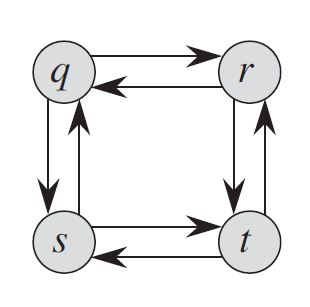
\includegraphics [scale = 0.5] {Graph.jpg}}
\caption{Задача о самом длинном невзвешенном пути}
\end{figure}
% <<<<картинка>>>>

Рассмотрим путь $q \rightarrow r \rightarrow t$, который является самым длинным простым путем $q \longrightarrow t$. 
Является ли путь $q\rightarrow r$ самым длинным путем $q \longrightarrow r$? Нет, поскольку простой путь $q \rightarrow s \rightarrow t \rightarrow r$ длиннее. 
Является ли путь $r \rightarrow t$ самым длинным путем $r \longrightarrow t$? Снова нет, поскольку простой 
путь $r \rightarrow q \rightarrow s \rightarrow t$ длиннее. Таким образом, в задаче о поиске самого длинного 
невзвешенного пути не возникает никаких оптимальных подструктур.

\section{Пример}

Требуется разложить натуральное число $n$ в сумму натуральных квадратов с наименьшим 
количеством слагаемых. К данной задаче применимо динамическое решение.

Создадим двумерный массив $a[n + 1][sqrt(n) + 1]$, номер столбца~--~это число, а коэффициенты в столбцах~--~это количество 
соответствующих квадратов в сумме. Номера строк ~--~это числа, квадраты которых могут присутствовать в разложении. 
Столбец под номером 0 обнулен. Теперь составим рекурентное соотношение.

$$F(x) = 1 + min(F(x - i^2))$$

Здесь $i$ пробегает все значения от 1 до sqrt(n). Минимальное значение берется по количеству 
натуральных квадратов в сумме. Массив можно заполнять как прямым, так и обратным ходом.

\end{document}
